\documentclass[twoside,10pt]{article}
\usepackage{/Users/bradenhoagland/latex/styles/toggles}
%\toggletrue{sectionbreaks}
%\toggletrue{sectionheaders}
\newcommand{\docTitle}{Math 323 - HW 10}
\usepackage{/Users/bradenhoagland/latex/styles/common}
\importStyles{modern}{rainbow}{boxy}

%\renewcommand{\theenumi}{\alph{enumi}}

\begin{document}
%\tableofcontents

% ------------------------------
% 10.15
% ------------------------------
\begin{exer}[10.15]
Spherical law of sines is compatible with Euclidean law of sines for very small $a,b,c$.
\end{exer}

The Taylor expansion of $\sin x$ is
\[
\sin x = x - \frac{x^{3}}{3!} - \frac{x^{5}}{5!} + \cdots,
\] so when $x$ is small, $\sin x \approx x$. Thus when $a,b,c$ are small,
\[
\frac{\sin a}{\sin A} = \frac{\sin b}{B} = \frac{\sin c}{\sin C} 
\] becomes approximately
\[
\frac{a}{\sin A} = \frac{b}{B} = \frac{c}{\sin C},
\] which is exactly the Euclidean law of sines.

\newpage

% ------------------------------
% 10.16
% ------------------------------
\begin{exer}[10.16]
Spherical law of cosines is compatible with Euclidean law of cosines for very small $a,b,c$.
\end{exer}

The Taylor expansion of $\cos x$ is
\[
\cos x = 1 - \frac{x^{2}}{2!} + \frac{x^{4}}{4!} - \cdots,
\] so when $x$ is small, $\cos x \approx 1 - x^2/2$. Thus when $a,b,c$ are small,
\[
	\cos c = \cos a \cos b + \sin a \sin b \cos C
\] becomes approximately
\begin{align*}
	1 - \frac{c^2}{2} &= \left( 1-\frac{a^{2}}{2}  \right)\left( 1-\frac{b^{2}}{2}  \right)+ab\cos C \\
	c^{2} &= a^{2}+b^2 + \frac{a^{2}b^{2}}{4} -2ab\cos C.
\end{align*}
But the $a^{2}b^2/4$ term goes to 0 much faster than the other terms, so this is approximately
\[
c^{2} = a^{2}+b^2-2ab\cos C,
\] 
which is exactly the Euclidean law of cosines.

\newpage

% ------------------------------
% 10.17
% ------------------------------
\begin{exer}[10.17]
Spherical law of sines and cosines for sphere of radius $\rho$.
\end{exer}

Suppose an arc on a sphere of radius $\rho$ is subtended by an angle $\theta$, then its arc length is $\theta \rho$. We can then transform it into an arc on the unit sphere viw the map $x \mapsto x/\rho$. Thus the modified laws of sines and cosines are
\[
	\frac{\sin (a/\rho)}{\sin A} = \frac{\sin (b/\rho)}{B} = \frac{\sin (c/\rho)}{\sin C}
\] and
\[
	\cos (c/\rho) = \cos (a/\rho) \cos (b/\rho) + \sin (a/\rho) \sin (b/\rho) \cos C
\] 

\newpage

% ------------------------------
% 10.21
% ------------------------------
\begin{exer}[10.21]
Derive Pythagorean theorem using Menelaus on the triangle in Figure 7.
\end{exer}

\begin{figure}[H]
	\centering
	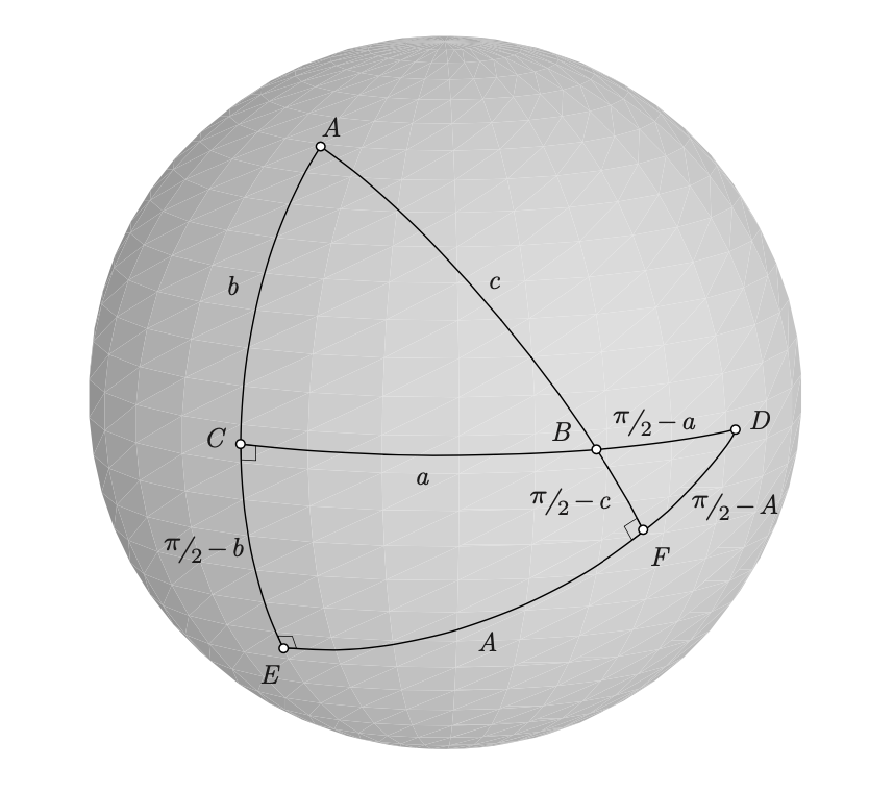
\includegraphics[scale=0.7]{fig/21.pdf}
	%\caption{}
\end{figure}

Since $D,E,F$ are collinear, Menelaus' theorem says
\[
\frac{\sin |AF|}{\sin |FB|} \frac{\sin |BD|}{\sin |DC|} \frac{\sin |CE|}{\sin |EA|} = -1.
\] But these are signed ratios, and $D$ does not lie on $BC$, so the LHS of the above equation has an additional negative sign. Thus plugging in the lengths of each line gives
\begin{align*}
	\sin|AF|\sin|BD|\sin|CE| &= \sin|FB|\sin|DC|\sin|EA| \\
	\sin\left( \frac{\pi}{2} \right) \sin\left( \frac{\pi}{2} -a \right)\sin\left( \frac{\pi}{2} -b \right) &= \sin\left( \frac{\pi}{2} -a \right)\sin\left( \frac{\pi}{2} \right)\sin\left( \frac{\pi}{2}  \right) \\
	\cos a \cos b &= \cos a,
\end{align*}
which is the spherical Pythagorean theorem.

\newpage

% ------------------------------
% 10.26
% ------------------------------
\begin{exer}[10.26]
State and prove Ceva's theorem on the sphere.
\end{exer}

\begin{thrm}[Spherical Ceva]
Suppose $\Delta ABC$ be a spherical triangle and let $D,E,F$ be points on $BC,AC,AB$, respectively. Then $AD,BE,CF$ are concurrent $\iff$ 
\[
\frac{\sin|AF|}{\sin|FB|} \frac{\sin|BD|}{\sin|DC|} \frac{\sin|CE|}{\sin|EA|} =1.
\] 
\end{thrm}

\begin{figure}[H]
	\centering
	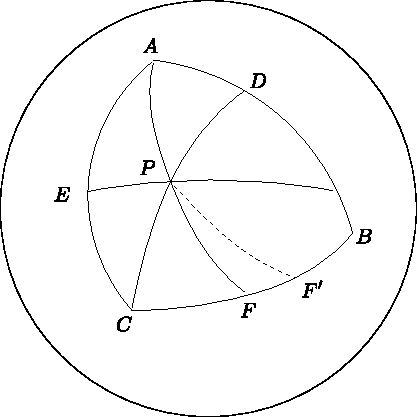
\includegraphics[scale=1]{fig/26.pdf}
	%\caption{}
\end{figure}

\textbf{Forward:} Suppose $BC,AC,$ and $AB$ are intersect at a common point $P$, then by Menelaus' theorem,
\[
	\frac{\sin|AF|}{\sin|FB|} \frac{\sin|BP|}{\sin|PE|} \frac{\sin|EC|}{\sin|CA|} = -1 = \frac{\sin|BD|}{\sin|DC|} \frac{\sin|CA|}{\sin|AE|} \frac{\sin|EP|}{\sin|PB|} .
\] Multiplying these two together and cancelling terms then gives
\[
\frac{\sin|AF|}{\sin|FB|}\frac{\sin|BD|}{\sin|DC|} \frac{\sin|CE|}{\sin|EA|} = 1.
\] 

\textbf{Backward:} Suppose $\frac{\sin|AF|}{\sin|FB|} \frac{\sin|BD|}{\sin|DC|} \frac{\sin|CE|}{\sin|EA|} =1$. Suppose $AD$ and $BE$ intersect at a point $P$, and let $CP$ intersect $AB$ at $F'$. By Menelaus' theorem and a similar argument as in the first half of the proof,
\[
\frac{\sin|AF'|}{\sin|F'B|} \frac{\sin|BD|}{\sin|DC|} \frac{\sin|CE|}{\sin|EA|} =1.
\] Then by our original assumption,
\begin{align*}
	\frac{\sin|AF'|}{\sin|F'B|} \frac{\sin|BD|}{\sin|DC|} \frac{\sin|CE|}{\sin|EA|} &= \frac{\sin|AF|}{\sin|FB|} \frac{\sin|BD|}{\sin|DC|} \frac{\sin|CE|}{\sin|EA|} \\
	\frac{\sin|AF'|}{\sin|F'B|} &= \frac{\sin|AF|}{\sin|FB|}.
\end{align*}
If $F' \neq F$, then $|AF'| = |AF|+x$ and $|F'B|=|FB|-x$. Plugging these into the above equality yields
\begin{align*}
	\frac{\sin|AF|+x}{\sin|FB|-x} &= \frac{\sin|AF|}{\sin|FB|} \\
	(\sin|AF|+x) \; \sin|FB| &= (\sin|FB|-x) \; \sin|AF| \\
	x(\sin|FB|+\sin|AF|) &= 0 \\
	x &= 0.
\end{align*}
This is a contradiction, so $F = F'$, meaning that $BC, AC,$ and $AB$ all intersect at $P$.

\newpage

% ------------------------------
% 10.35
% ------------------------------
\begin{exer}[10.35]
	Edge length of the polygons in the semiregular tiling $(3,3,5,5)$ of the unit sphere.
\end{exer}

	There are two pentagons and 2 triangles per vertex, and their angles at each vertex must sum to $2\pi$ in order for it to be a tiling. Since the tiling is semiregular, by symmetry we know the angles of 1 pentagon and 1 triangle at each vertex sum to $\pi$, i.e. form a portion of a geodesic. We can repeat this argument to find a sequence of edges forming an entire eodesic on the sphere.

	Thus this problem reduces to counting the number of edges in a geodesic along the ``great circles" of a truncated icosahedron. There are 10 edges, so since the length of a geodesic on a unit sphere is $2\pi$, each edge must have length 
	\[
	\frac{2\pi}{10} = \frac{\pi}{5} .
	\] 

\newpage

% ------------------------------
% 10.36
% ------------------------------
\begin{exer}[10.36]
	Percentage of area of sphere covered by triangles in the semiregular tiling $(3,3,5,5)$.
\end{exer}

By the previous exercise, each triangle has sides of length $\pi/5$. Since they're regular triangles, each inner angle is the same; denote it by $\theta$. Then by the spherical law of cosines,
\begin{align*}
	\cos\left( \frac{\pi}{5}  \right) &= \cos^2\left( \frac{\pi}{5}  \right) + \sin^2\left( \frac{\pi}{5}  \right) \cos \theta \\
	\frac{1+\sqrt{5} }{4} &= \frac{3+\sqrt{5} }{8} + \frac{5-\sqrt{5} }{8} \cos \theta \\
	\cos \theta &= \frac{2+2\sqrt{5} -3-\sqrt{5} }{5-\sqrt{5} } \\
	\cos \theta &= \frac{1}{\sqrt{5} } .
\end{align*}
Then the area of each triangle in the tiling is $3 \theta - \pi = 3\arccos(1/\sqrt{5} )-\pi$. Since the entire sphere has area $4\pi$, the percentage of the sphere covered by triangles is
\[
	\frac{20 \big( 3\arccos(1/\sqrt{5} )-\pi \big)}{4\pi} \approx 28.62\%.
\] 

\newpage

\end{document}
